%-------------------------
% Resume for Postdoc Application
% Author : Haoyuan Liu
%------------------------

\documentclass[letterpaper,11pt]{article}

\usepackage{graphicx}
\usepackage{latexsym}
\usepackage[empty]{fullpage}
\usepackage{titlesec}
\usepackage{marvosym}
\usepackage[usenames,dvipsnames]{color}
\usepackage{verbatim}
\usepackage{enumitem}
\usepackage[hidelinks]{hyperref}
\usepackage{microtype}
\usepackage{fancyhdr}
\usepackage[english]{babel}
\usepackage{tabularx}
\input{glyphtounicode}

%----------FONT OPTIONS----------
\usepackage[default]{sourcesanspro}

\pagestyle{fancy}
\fancyhf{} 
\fancyfoot{}
\renewcommand{\headrulewidth}{0pt}
\renewcommand{\footrulewidth}{0pt}

% Adjust margins
\addtolength{\oddsidemargin}{-0.5in}
\addtolength{\evensidemargin}{-0.5in}
\addtolength{\textwidth}{1in}
\addtolength{\topmargin}{-.5in}
\addtolength{\textheight}{1.0in}

\urlstyle{same}

\raggedbottom
% \raggedright
\setlength{\tabcolsep}{0in}

% Sections formatting
\titleformat{\section}{
  \vspace{-4pt}\scshape\raggedright\large
}{}{0em}{}[\color{black}\titlerule \vspace{-5pt}]

% Ensure that generate pdf is machine readable/ATS parsable
\pdfgentounicode=1

%-------------------------
% Custom commands
% \newcommand{\resumeItem}[1]{
%   \item\small{
%     {#1 \vspace{-2pt}}
%   }
% }
\newcommand{\resumeItem}[1]{
  % Use a smaller, centered bullet to match your style
  \item[$\vcenter{\hbox{\tiny$\bullet$}}$]\small{
    {#1 \vspace{-2pt}}
  }
}

\newcommand{\resumeItemF}[1]{
  \item[] \small{
    {#1 \vspace{-2pt}}
  }
}

\newcommand{\resumeSubheading}[4]{
  \vspace{-2pt}\item
    \begin{tabular*}{0.97\textwidth}[t]{l@{\extracolsep{\fill}}r}
      \textbf{#1} & #2 \\
      \textit{\small#3} & \textit{\small #4} \\
    \end{tabular*}\vspace{-7pt}
}

\newcommand{\resumeProjectHeading}[2]{
    \item
    \begin{tabular*}{0.97\textwidth}{l@{\extracolsep{\fill}}r}
      \small#1 & #2 \\
    \end{tabular*}\vspace{-7pt}
}

\newcommand{\resumeSubItem}[1]{\resumeItem{#1}\vspace{-4pt}}
\renewcommand\labelitemii{$\vcenter{\hbox{\tiny$\bullet$}}$}
\newcommand{\resumeSubHeadingListStart}{\begin{itemize}[leftmargin=0.15in, label={}]}
\newcommand{\resumeSubHeadingListEnd}{\end{itemize}}
\newcommand{\resumeItemListStart}{\begin{itemize}}
\newcommand{\resumeItemListEnd}{\end{itemize}\vspace{-5pt}}

%-------------------------------------------
%%%%%%  CV STARTS HERE  %%%%%%%%%%%%%%%%%%%%%%%%%%%%

\begin{document}

%----------HEADING----------
% \begin{center}
%     \textbf{\Huge \scshape Haoyuan Liu} \\ \vspace{5pt}
%     \small 
%     liuhaoyuan [at] akane.waseda.jp $|$
%     \href{https://github.com/NuayHL}{\underline{github.com/NuayHL}}
% \end{center}

\noindent
\begin{minipage}[c]{0.70\textwidth}
    \raggedright
    \textbf{\Huge \scshape Haoyuan Liu} \\ \vspace{5pt}
    \small
    liuhaoyuan [at] akane.waseda.jp \\
    \href{https://github.com/NuayHL}{\underline{github.com/NuayHL}}
\end{minipage}%
\hfill
\begin{minipage}[c]{0.25\textwidth}
    \raggedleft
    % Upload your photo (e.g., photo.jpg) to the project folder
    % Change 'photo.jpg' to your actual file name
    % Adjust 'width' to resize the image (e.g., 2.5cm or 0.8\linewidth)
    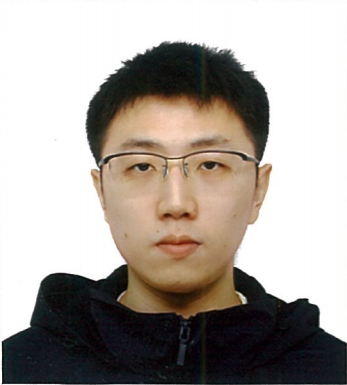
\includegraphics[width=3.4cm]{figure.png}
\end{minipage}

%-----------EDUCATION-----------
\section{Education}
  \resumeSubHeadingListStart
    \resumeSubheading
      {Waseda University}{Tokyo, Japan}
      {Ph.D. in Computer Science and Communications Engineering}{Sep. 2023 -- Sep. 2026}
      \resumeItemListStart
        \resumeItem{Advisor: Prof. Hiroshi Watanabe (\href{https://www.ams.giti.waseda.ac.jp/}{Advance Multimedia Systems(AMS) Lab})}
        \resumeItem{Research Focus: Multi-modal Object Detection, Tiny Object Detection}
      \resumeItemListEnd

    \resumeSubheading
      {Waseda University}{Tokyo, Japan}
      {M.Eng. in Computer Science and Communications Engineering (GPA: 3.8/4.0)}{Sep. 2021 -- Sep. 2023}
      \resumeItemListStart
        \resumeItem{Advisor: Prof. Hiroshi Watanabe (\href{https://www.ams.giti.waseda.ac.jp/}{Advance Multimedia Systems(AMS) Lab})}
        \resumeItem{Research Focus: Object Detection, Pedestrian Detection, Dense Detection}
      \resumeItemListEnd

    \resumeSubheading
      {Beihang University (BUAA)}{Beijing, China}
      {B.S. in Information and Computing Science (School of Mathematical Sciences)(GPA: 3.2/4.0)}{Sep. 2016 -- Jul. 2020}
      \resumeItemListStart
        \resumeItem{Core Courses: Mathematical Logic, Optimization Theory, Probability Theory, Real/Complex Analysis, Functional Analysis}
      \resumeItemListEnd
      
    % Exchange Programs
    \resumeSubheading
      {National University of Ireland, Maynooth}{Maynooth, Ireland}
      {Exchange Student (Core courses: Algebraic Topology, Differential Geometry, PDE)}{Sep. 2018 -- Dec. 2018}

    % \resumeSubheading
    %   {University College London (UCL)}{London, UK}
    %   {Summer Exchange (Academic Writing)}{Jul. 2017 -- Aug. 2017}

  \resumeSubHeadingListEnd

\section{Research Interests}
\small
\begin{itemize}[leftmargin=0.15in, label={}]
\item \textbf{Visual Perception and Scene Understanding:}
Visual perception problems in complex real-world scenarios, including object detection, segmentation, scene-graph generation, and fine-grained recognition, with a particular focus on representation stability and generalization under small-object, dense, and cross-scale settings, gradually extending to open-vocabulary detection and language-guided localization.
\item \textbf{Self-Supervised Visual Representation Learning:}
Transformer-based self-supervised visual learning methods (e.g., the DINO series), with an emphasis on learning semantically consistent representations under unlabeled or weakly labeled settings, and their transfer to downstream detection and localization tasks.
\item \textbf{Multimodal Perception and Agent Systems:}
Multimodal visual representation learning and cross-modal alignment, covering perception tasks such as RGB–infrared/thermal image fusion and remote sensing image understanding, with a further focus on agent systems built upon multimodal large models (in particular compact 4B–8B vision–language models with open-vocabulary grounding), including vision–language joint reasoning, referring localization, task planning, and tool use, as well as the stability and reliability of perceptual outputs in downstream decision-making.
\end{itemize}


%-----------PUBLICATIONS-----------
\section{Publications}
{\footnotesize $^{\dagger}$ Corresponding Author}
  \resumeSubHeadingListStart
    \resumeItem{\textbf{Haoyuan Liu}, Hiroshi Watanabe. "InterpIoU: Robust Bounding Box Regression Loss within an Interpolation-Based IoU Framework." \textit{Neurocomputing}, Vol. 666, 2026.}
    
    \resumeItem{\textbf{Haoyuan Liu}, Hiroshi Watanabe. "GSA: Guided Supervised Attention for Enhancing Real-Time Dense Object Detection via Parameter-Free Scheme." \textit{Journal of Electronic Imaging}, Vol. 33(6), Nov. 2024.}

    \resumeItem{\textbf{Haoyuan Liu}, Hiroshi Watanabe. "Feature Transfer Block for Feature Fusion in Lightweight Object Detectors." \textit{IEEE 12th Global Conference on Consumer Electronics (GCCE)}, Oct. 2023.}

    \resumeItem{Ziyue Zeng, Xun Su, \textbf{Haoyuan Liu}, Bingyu Lu, Yui Tatsumi, Hiroshi Watanabe. "GVCC: Zero-Shot Video Compression via Codebook-Driven Stochastic Rectified Flow." \textit{Conference on Neural Information Processing Systems (NeurIPS)}, Dec. 2026. Accepted (Poster).}

    \resumeItem{Bingyu Lu, \textbf{Haoyuan Liu}$^{\dagger}$, Ziyue Zeng, Hiroshi Watanabe. "WMPF: Wavelet-Decoupled Discrepancy Mitigation and Detail-Preserving Fusion for RGB--IR Object Detection." \textit{IEEE/CVF Winter Conference on Applications of Computer Vision (WACV)}, 2027. Accepted (Round 2).}

    \resumeItem{Gaosiheng Chen, Bingyu Lu, \textbf{Haoyuan Liu}, Hiroshi Watanabe. "Partial Cross-Modal Channel Injection for RGB-Infrared Spatial Alignment." \textit{International Workshop on Advanced Image Technology (IWAIT)}, Jan. 2027. Accepted.}

    \resumeItem{Mohan Yin, \textbf{Haoyuan Liu}$^{\dagger}$, Hongrui Fan, Bingyu Lu, Hiroshi Watanabe. "TMSF-YOLO: Two-Round Multi-Scale Fusion with Semantic Feedback for Small-Object Detection." \textit{IEEE International Conference on Systems, Man, and Cybernetics (SMC)}, Bellevue, WA, USA, Oct. 2026. Accepted Jun. 2026.}

    \resumeItem{Bingyu Lu, \textbf{Haoyuan Liu}$^{\dagger}$, Hiroshi Watanabe. "A Foreground-Background Differentiated Fusion Model for RGB-Infrared Object Detection." \textit{IEEE International Conference on Systems, Man, and Cybernetics (SMC)}, Bellevue, WA, USA, Oct. 2026. Accepted Jun. 2026.}

    \resumeItem{Ziyue Zeng, Yupei Guo, \textbf{Haoyuan Liu}, Dingjie Peng, Hiroshi Watanabe. "Time Step Generating: A Universal Synthesized Deepfake Image Detector." \textit{ACM Multimedia Asia (MMAsia)}, Dec. 2025.}

    \resumeItem{Gaosiheng Chen, Bingyu Lu, \textbf{Haoyuan Liu} and Hiroshi Watanabe. "Local Feature Calibration and Adaptive Fusion for Small-Object RGB-Infrared Object Detection" \textit{IEEE GCCE}, Oct. 2026.}

    \resumeItem{Yihua Jing, \textbf{Haoyuan Liu} and Hiroshi Watanabe. "Semantic-Driven Backbone Enhancement for Small Object Detection in UAV Imagery" \textit{IEEE GCCE}, Oct. 2026.}

    \resumeItem{Wotong Li, \textbf{Haoyuan Liu} and Hiroshi Watanabe. "Bridging Gaussian Representation and Real-Time Detection via Cholesky Parameterization" \textit{IEEE GCCE}, Oct. 2026.}

    \resumeItem{Bingyu Lu, \textbf{Haoyuan Liu}, Hiroshi Watanabe. "Enhancing RGB-Infrared Object Detection: A Frozen Backbone Approach with Multi-Receptive Field Attention." \textit{The Visual Computer (Springer Nature)}. 2026}
  
    \resumeItem{Hongrui Fan, \textbf{Haoyuan Liu}, Hiroshi Watanabe. "A Lightweight Channel Bias for Small Object Detection in Aerial Images." \textit{International Workshop on Advanced Image Technology (IWAIT)}, Jan. 2026.}

    \resumeItem{Hongrui Fan, \textbf{Haoyuan Liu}, Hiroshi Watanabe. "Enhancing Object Detection with Non-Local Modules in the Feature Pyramid Network." \textit{IEEE GCCE}, Oct. 2024.}

    \resumeItem{Jiu Yi, \textbf{Haoyuan Liu}, Hiroshi Watanabe. "Distilled RSN: Lightweight Pose Estimation Using Knowledge Distillation." \textit{IEEE GCCE}, Oct. 2024.}
    
    \resumeItem{Jiahao Liu, \textbf{Haoyuan Liu}, Hiroshi Watanabe. "Video Salient Object Detection Using Multi-Scale Self-Attention." \textit{IEEE GCCE}, Oct. 2023.}
  \resumeSubHeadingListEnd
  
\noindent\textbf{Manuscripts Under Review \& Preparation}
\vspace{-5pt}
  \resumeSubHeadingListStart
    \resumeItem{\textbf{Haoyuan Liu}, Mohan Yin, Bingyu Lu, Wen Yang, Ziyue Zeng, Hiroshi Watanabe. "The Supervision Ceiling: Scale Aware Calibration for Reliable Small Object Detection" Submitted to Pattern Recognition.}

    \resumeItem{\textbf{Haoyuan Liu}, Tianshui Chen, Hiroshi Watanabe, Liang Lin. "Geometry-Adaptive Feature Enhancement and Contextual Diffusion for Small Object Detection in UAV Imagery." Submitted to ISPRS Journal of Photogrammetry and Remote Sensing.}

    % \resumeItem{Bingyu Lu, \textbf{Haoyuan Liu}, Hiroshi Watanabe. "A Foreground-Background Differentiated Fusion Model for RGB-Infrared Object Detection." Under review at \textit{ICASSP 2026}.}
  \resumeSubHeadingListEnd

%-----------TEACHING & MENTORSHIP-----------
\section{Teaching \& Mentorship Experience}
  \resumeSubHeadingListStart
    \resumeSubheading
      {Waseda University}{Tokyo, Japan}
      {Teaching Assistant (TA)}{Sep. 2024 -- Sep. 2026}
      \resumeItemListStart
        \resumeItem{Delivered selected lectures and course modules in \textit{Multimedia and Standards} and \textit{Image Processing}.}
      \resumeItemListEnd

    \resumeSubheading
      {AMS Laboratory, Waseda University}{Tokyo, Japan}
      {Group Leader of Recognition Research Group}{Sep. 2023 -- Sep. 2026}
      \resumeItemListStart
        \resumeItem{Supervised daily research activities of undergraduate and master's students.}
      \resumeItemListEnd
  \resumeSubHeadingListEnd

%-----------RESEARCH EXPERIENCE-----------

\section{Research Experience}
  \resumeSubHeadingListStart

    \resumeSubheading
    {The Hong Kong Polytechnic University}{Hong Kong SAR, China}
    {\quad Postdoctoral Researcher, Lumen Lab}{Oct. 2026 -- Present}
    \resumeItemListStart
        \resumeItem{Research focus: text-to-CAD program synthesis with compact language models, open-vocabulary detection and language-guided localization, and multimodal agent systems.}
    \resumeItemListEnd
    \vspace{0.1cm}

    \resumeSubheading
    {China Telecom Beijing Research Institute}{Beijing, China}
    {\quad Research Intern(Remote), AI R\&D Center}{Apr. 2023 -- Dec. 2024}
    \resumeItemListStart
        \resumeItem{Conducted research on Trusted AI evaluation, AI compliance platforms, and safety analysis of large language models.}
    \resumeItemListEnd
% ---------------------------------------------------------------------------
% Research Experience Section
% ---------------------------------------------------------------------------
    \vspace{0.1cm}

\resumeSubheading
  {Towards Robust Small Object Detection: Multi-Stage Pipeline Optimization}{Waseda University}
  {\quad Ph.D. Research Topic}{Sep. 2023 -- Sep. 2026}
  \resumeItemListStart
    \resumeItemF{Small object detection remains a core challenge due to weak features, unreliable localization signals, and unstable optimization, especially in dense aerial imagery. During my Ph.D., I adopted one-stage detectors as the primary platform and systematically investigated the signal reliability and optimization stability issues that small objects face across \textbf{feature extraction, label assignment, and supervision optimization}. This line of research forms a coherent multi-stage pipeline optimization framework, progressing from feature representation enhancement, through scale-aware matching, to supervision signal refinement.}
    
    \resumeItem{\textbf{Feature Representation (Published / Under Review):} Addressing the systematic degradation of small object features in the standard CNN-FPN paradigm, designed a \textbf{Lightweight Contextual and Local Feature Enhancement Framework (CLFE)} that jointly improves feature extraction and fusion from two perspectives: fine-grained local detail preservation and cross-scale contextual interaction regulation. Related results published in \textit{\textbf{JEI}} and \textit{\textbf{IEEE GCCE}}; a full framework paper is under review at \textit{\textbf{ISPRS JPRS}}.}
    
    \vspace{0.1cm}
    
    \resumeItem{\textbf{Label Assignment (Under Review):}  Revisited task-aligned label assignment from the perspective of training signal reliability, revealing that fixed alignment formulations suffer from matching oscillation for small objects due to noisy localization signals and geometrically unstable similarity metrics. Proposed \textbf{USAA}, a unified scale-adaptive assignment framework that dynamically reweights task signals and introduces a bounded-tolerance geometric similarity metric, significantly improving matching stability for small objects. Paper in preparation for submission.}
    
    \vspace{0.1cm}
    
    \resumeItem{\textbf{Regression Loss (Published):} Proposed \href{https://github.com/NuayHL/interpiou}{\underline{\textbf{InterpIoU}}}, an interpolation-based IoU loss that eliminates handcrafted geometric penalties while providing stable, IoU-aligned gradients for small object localization. Published in \textit{\textbf{Neurocomputing}} and adopted by multiple follow-up works.}
  \resumeItemListEnd


  
      \vspace{0.2cm}
      \resumeSubheading
      {Remote Sensing Image Fusion based on CNN}{Beihang University}
      {\quad Bachelor's Graduation Project}{Feb. 2020 -- Jul. 2020}
      \resumeItemListStart
        \resumeItem{Developed a CNN-based pansharpening method using ResNet architectures and self-supervised learning for high-resolution remote sensing imagery.}
      \resumeItemListEnd

  \resumeSubHeadingListEnd


%-----------SKILLS-----------

%\section{Technical Skills}
%\begin{itemize}[leftmargin=0.15in, label={}]
%\small{
%\item \textbf{Programming:} Python (proficient), C / C++
%\item \textbf{Deep Learning:} Proficient with PyTorch (Advanced, Custom C++/CUDA Extensions), Ultralytics (YOLO) and MMCV/MMDetection frameworks; experienced in independently building end-to-end object detection training pipelines.
%\item \textbf{Tools and Systems:} Linux, Git, LaTeX, Docker
%}
% \end{itemize}

%-----------HONORS AND AWARDS-----------
%\section{Honors and Awards}
%  \resumeSubHeadingListStart
%    \resumeProjectHeading
%      {\textbf{CSC Scholarship} (China Scholarship Council for PhD Study)}{2023}
%    \resumeProjectHeading
%      {\textbf{Meritorious Winner}, MCM/ICM (Mathematical Contest in Modeling)}{2019}
%    \resumeProjectHeading
%      {\textbf{CSC Outstanding Undergraduate Scholarship} (China Scholarship Council)}{2018}
%  \resumeSubHeadingListEnd

\end{document}